
\subsubsection{Reference Sorption Coefficient Sensitivity}

In the parametric analysis of \Cyder performance, it was shown that sorption 
sensitivity behavior closely matched that of the \gls{GDSM} sensitivity 
behaviors. Specifically, in Figure \ref{fig:}, increasing the retardation 
coefficient results in a smooth but dramatic turnover. 

\begin{figure}[ht]
\centering
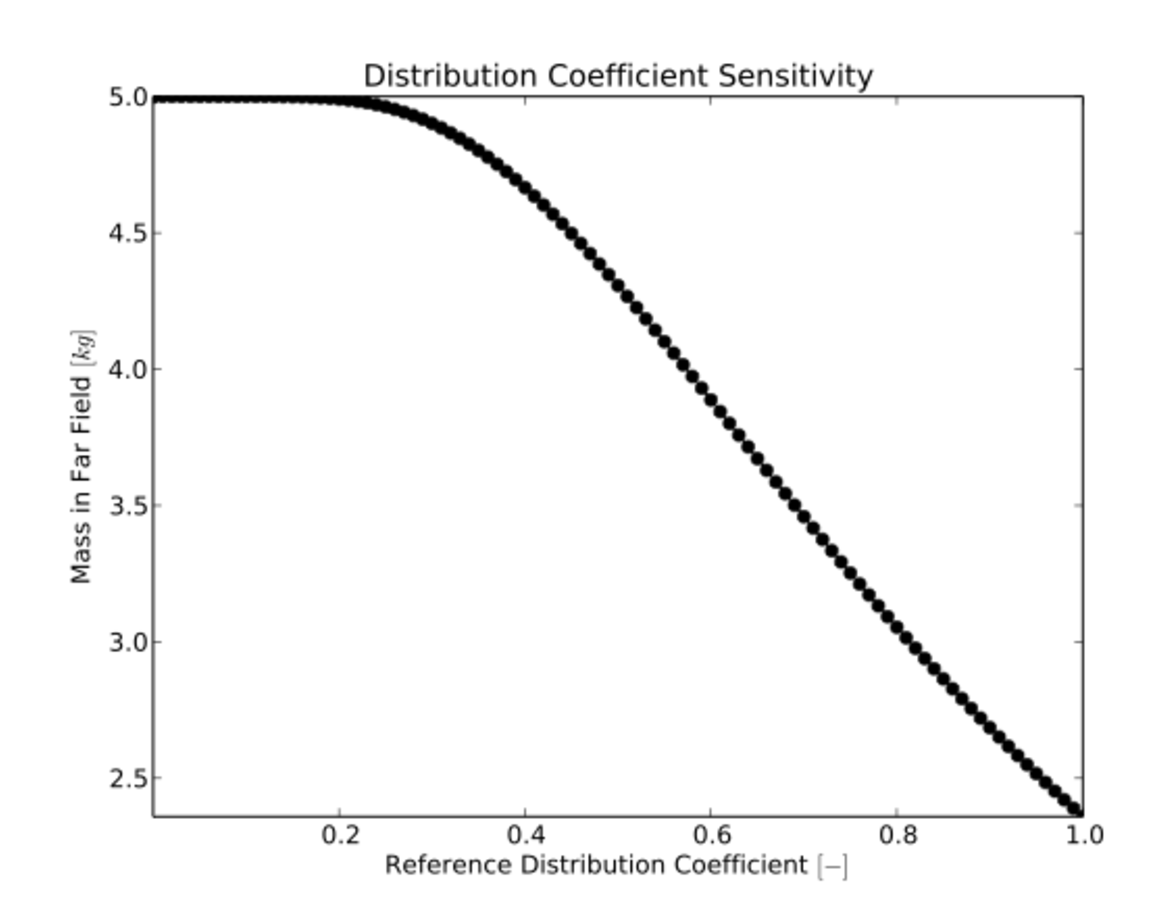
\includegraphics[width=0.7\linewidth]{./chapters/demonstration/bench/kd.eps}
\caption{$K_d$ factor sensitivity in the \Cyder tool for an arbitrary isotope 
assigned a variable $K_d$ coefficient. (NOTE: I know the first three data 
points are funky. I know how to deal with it, I just have to re-run this 
sim-set.)}
\label{fig:kd_result}
\end{figure}
